\documentclass[tikz]{standalone}

\colorlet{FilledSurface}{blue!20}
\colorlet{FilledSurfaceGroupOne}{blue!20}
\colorlet{FilledSurfaceGroupTwo}{red!20}
\colorlet{FilledSurfaceGroupThree}{green!20}
\colorlet{FilledSurfaceGroupFour}{magenta!20}
\colorlet{FormulaBackground}{green!10}
\colorlet{FormulaFrame}{green}


\usetikzlibrary{calc, decorations.markings, intersections}

\tikzset{
    mark rect/.style={
        decoration={markings, mark=at position 0.5 with {
                \draw[draw=black, fill=white] (-6pt,-2pt) rectangle (6pt,2pt);
        }}, postaction={decorate}
    },
    mark one circle/.style={
        decoration={markings, mark=at position 0.5 with {
                \draw[fill=white] (0,0) circle (2pt);
        }}, postaction={decorate}
    },
    mark two circles/.style={
        decoration={markings, mark=at position 0.5 with {
                \draw[fill=white] (-2pt,0) circle (2pt);
                \draw[fill=white] (2pt,0) circle (2pt);
        }}, postaction={decorate}
    }
}

\begin{document}
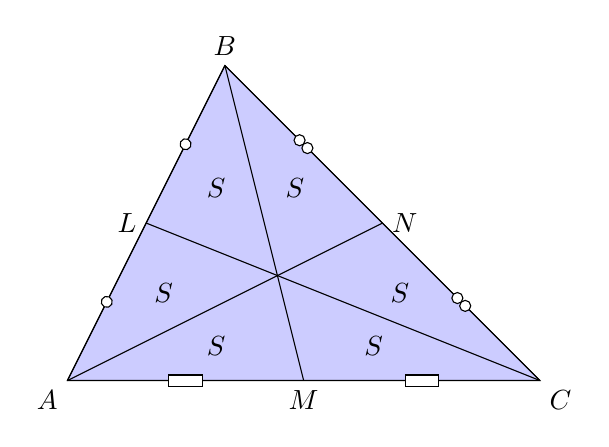
\begin{tikzpicture}

    \coordinate (A) at (0,0);
    \coordinate (B) at (2,4);
    \coordinate (C) at (6,0);

    \draw [fill=FilledSurfaceGroupOne] (A) node [below left]{$A$}
    -- (B) node [above]{$B$}
    -- (C) node [below right]{$C$}
    -- cycle;

    \coordinate (M) at ($(A)!0.5!(C)$);
    \coordinate (N) at ($(B)!0.5!(C)$);
    \coordinate (L) at ($(A)!0.5!(B)$);

    % Dibujar medianas
    \draw[name path = BM] (B) -- (M) node [below] {$M$};
    \draw[name path = CL] (C) -- (L) node [left] {$L$};
    \draw (A) -- (N) node [right] {$N$};
    \path [name intersections={of=BM and CL, by=I}];

    % Añadir marcadores a los segmentos determinados por las medianas.
    \draw[mark rect] (A) -- (M);
    \draw[mark rect] (C) -- (M);
    \draw[mark one circle] (A) -- (L);
    \draw[mark one circle] (B) -- (L);
    \draw[mark two circles] (B) -- (N);
    \draw[mark two circles] (C) -- (N);

    \node at (barycentric cs:A=1,I=1,L=1) {$S$};
    \node at (barycentric cs:L=1,I=1,B=1) {$S$};
    \node at (barycentric cs:B=1,I=1,N=1) {$S$};
    \node at (barycentric cs:N=1,I=1,C=1) {$S$};
    \node at (barycentric cs:C=1,I=1,M=1) {$S$};
    \node at (barycentric cs:M=1,I=1,A=1) {$S$};

\end{tikzpicture}
\end{document}

% Si AN, BM y CL son medianas:
